\chapter{Derived Schema of Symmetric Crypto}

\section{SHA3 Derived Schemes}
\begin{flushleft}

    Abbiamo detto che una funzione hash ritorna come output una quantità fissa di bytes. Se quindi ci dovesse essere la necessità di avere \textbf{meno dati}, allora ``basterebbe'' \textbf{troncare} il \textbf{\textit{digest}}, nel caso opposto invece possiamo ri-progettare un algoritmo simile a \textbf{CTR} e invocarlo più volte, il che, però, porterebbe molto più sforzo da parte degli sviluppatori e rischierebbe di introdurre delle vulnerabilità nel codice.
    
    \smallskip

    È stato quindi introdotto il \textbf{\textit{eXtendible Output Function - XOF}} ovvero una \textbf{\textit{variable-length hash funciton}}.

    \smallskip

    \textcolor{red}{\textbf{\textit{cSHAKE}}}: è una variante di SHA3 e accetta i seguenti input addizionali:
    \begin{enumerate}[nosep]
        \item \textbf{\textit{output length}}: definisce la dimensione del digest.
        \item \textbf{\textit{custom string}}: specializza l'esecuzione della funzione \textit{hash} per un certo \textbf{contesto}. È molto utile per \textbf{\textit{domain (contest) separation}}.
    \end{enumerate}

    \begin{figure}[h]
        \centering
        \begin{minipage}[c]{0.45\textwidth}
            \textbf{cSHAKE128} ha 128bit di sicurezza ed è una variante di SHA3-256.
        \end{minipage}
        \hfill
        \begin{minipage}[c]{0.45\textwidth}
            \textbf{cSHAKE256} ha 256bit di sicurezza ed è una variante di SHA3-512.
        \end{minipage}
    \end{figure}

    \smallskip

    \textcolor{red}{\textbf{\textit{TupleHash}}}: è una funzione \textit{hash} ha delle interfacce con un astrazione \textit{high-level}, infatti permette di accettare una \textbf{lista di valori} e una \textbf{\textit{custom string}} come input. È un \textit{wrap} di \textbf{cSHAKE} che permette di supportare delle liste come valore di input, alle quali viene prima applicata una codifica in modo non ambiguo assegnando ad ogni elemento un'unica sequenza di bit - bitstring - poi verrà passata a cSHAKE come input. La \textit{custom string} ha un valore di default al quele viene concatenato quello dell'utente: \textit{TupleHash}. È utilizzata per evitare ambiguità di concatenazione. È deterministica e strutturate, utile in contesti crittografici dove serve un hash sicura su strutture dati complesse.

    \smallskip

    \textcolor{red}{\textbf{\textit{ParallelHash}}}: è progettato per per sfruttare ambienti paralleli (multi-core, GPU, ecc.) allo scopo di accelerare il calcolo dell'hash su grandi quantità di dati.
    \begin{enumerate}[nosep]
        \item i dati vengono suddivisi in blocchi.
        \item per ogni blocco viene calcolato il \textit{digest} in parallelo.
        \item i \textit{digest} dei vari blocchi (\textbf{\textit{digest parziali}}) vengono poi combinati per calcolare un \textit{digest} finale sugli output precedenti, ottenendo il digest complessivo del messaggio.
    \end{enumerate}
    Questo approccio ricorda un \textbf{\textit{Merkle Hash Tree - MHT}} dove le foglie sono gli hash dei blocchi e il nodo radice è l'hash finale ottenuto dall'unione degli hash sottostanti. \\ 
    \textbf{\textit{N.B.}} esistono funzioni di hash - ad esempio \textbf{Blake2} - che hanno meccanismi interni che la rendono automaticamente parallelizzabili anche senza un architettura come quella di ParallelHash.

    \smallskip

    \textcolor{red}{\textbf{\textit{MAC for SHA3}}}: \textbf{SHA3} è stato progettato e sviluppato per evitare \textbf{\textit{length extesion attack}} è quindi possibile non utilizzare l'\textbf{HMAC} basato su SHA3, in quanto ci sarebbe dell'\textit{overhead} inutile, ma sarebbe possibile avere un MAC che si basa su SHA3 come:

    {\centering
        \textbf{tag} $\leftarrow$ \textcolor{red}{\textbf{SHA3(k || message)}}
    \par}

    Bisogna solo fare attenzione a non utilizzare questo metodo con funzioni di hash che utilizzano come primitiva la costruzione \textbf{Merkle-Damgard} - per SHA2 utilizzare HMAC.

    \smallskip

    \textcolor{red}{\textbf{\textit{KMAC}}}: è un \textbf{MAC} a dimensione variabile che si basa su \textbf{cSHAKE}. Come input \textbf{KMAC} richiede:
    \begin{enumerate}[nosep]
        \item una \textbf{chiave} segreta $k$.
        \item un \textbf{messaggio} $m$.
        \item una \textbf{\textit{custom string}} che verrà concatenato al valore di default \textit{KMAC}.
        \item una \textbf{lunghezza} desiderata dell'output.
    \end{enumerate}
    Vengono combinati, in maniera sicura, la chiave, il messaggio e la \textit{custom string}, il tutto viene passato in input a cSHAKE che ne calcola il \textbf{tag}.

    \begin{figure}[h]
        \centering
        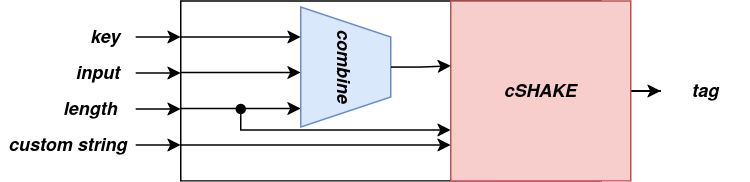
\includegraphics[width=0.75\textwidth]{img/kmac.png}
    \end{figure}
\end{flushleft}

\newpage

\section{Key Derivation Function}

\begin{flushleft}
    Molti schemi crittografici e protocolli spesso richiedono almeno due chiavi segrete non correlate, ma di contro si cerca di dover gestire un'unica chiave durante le procedure di \textit{key management} e di \textit{key distribution}.

    \smallskip

    Le \textbf{\textit{KDF}} sono funzioni che permetto di generare più \textit{pseudo-random keys} partendo da una singola chiave. Le \textbf{KDF} sono simili a delle \textbf{PRF}, infatti, prendono in input una singola stringa segreta e in maniera \textbf{deterministica} in output verrà generata una sequenza più lunga di dati pseudo-random che possono essere utilizzate come chiavi indipendenti e multiple. A differenza dei \textbf{PRF}, però, la \textbf{KDF} è progettata per generare una sequenza più corta e in più possono supportare altre funzionalità - ad esempio \textbf{\textit{input string}}, \textbf{\textit{explicit salting}} e lo \textbf{\textit{scoping}}. \\
    È possibile re-implementare una \textbf{KDF} utilizzando come primitive \textit{block cipher}, \textit{stream cipher}, MAC o \textit{hash function}. Esistono, però, delle \textbf{KDF} stardandizzate dal NIST, la più popolare è chiamata \textbf{HKDF} e si basa su un \textbf{HMAC}.

    \smallskip

    Un'implementazione di alto livello di una \textbf{KDF} ha due funzioni interne:
    \begin{enumerate}[nosep]
        \item \textcolor{red}{\textbf{\textit{extraction}}}: che dato una \textit{secret string} - possibilmente \textbf{non uniforme} e con un \textbf{alto livello di entropia} (comparabile con il \textit{security level}) - genera \textbf{una} chiave segreta (pseudo-random) uniforme.
        \item \textcolor{blue}{\textbf{\textit{expansion}}}: data una \textit{secret key} uniforme genera una chiave \textbf{pseudorandom} più lunga - ad esempio generare una chiave da un'altra per \textit{key scoping} o \textit{key rotation}
    \end{enumerate}

    \begin{figure}[h]
        \centering
        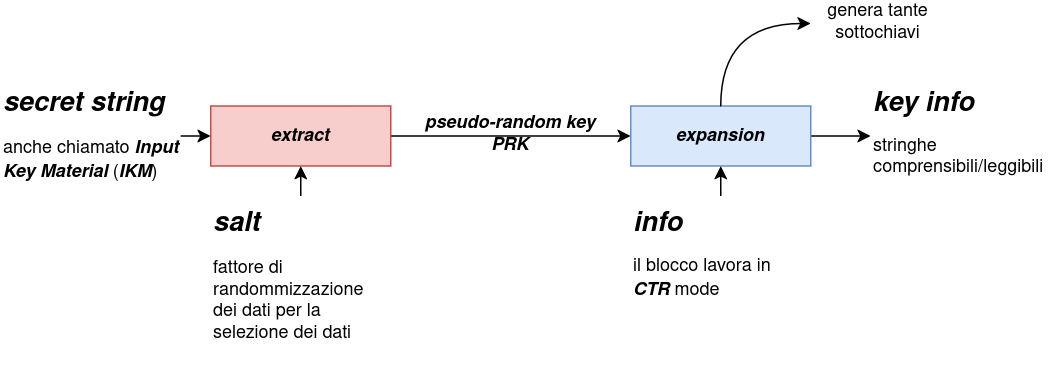
\includegraphics[width=\textwidth]{img/kdf.png}
    \end{figure}

    Una \textbf{KDF} è un metodo sicuro per derivare una chiave segreta anche se l'input è una string non uniforme (uniforme = alta entropia), ma l'input deve avere alta entropia e, ad esempio, una password per definizione - segreto che può essere ricordato da un umano - raramente ha abbastanza entropia $\rightarrow$ \textbf{\textit{Password-Based Key Derivation}} anche note come \textbf{\textit{Password Hashing}}. Nel caso in cui si abbia già un segreto random binario possiamo \textit{bypassare} il blocco di \textbf{\textit{extract}} e passare subito all'\textbf{\textit{expansion}}. Una \textbf{KDF} può dare funzionalità aggiuntive tra cui: aggiungere \textbf{randomicità} e aggiungere \textit{scoping information} (ad esempio per fare \textit{domain separation}).

    \smallskip

    Gli input di una \textbf{KDF} sono:
    \begin{itemize}[nosep]
        \item l'\textbf{algoritmo}: la funzione di hash interna (SHA256).
        \item \textbf{\textit{string}}: è la stringa segreta (con alta entropia).
        \item \textbf{\textit{length}}: lunghezza desiderata per la chiave derivata - simile all'input della dimensione per \textbf{XOF} e \textbf{KMAC}.
        \item \textbf{\textit{info}}: è una stringa che rappresenta il contesto per la separazione dei domini.
        \item \textbf{\textit{salt}}: è una stringa, è opzionale, se viene utilizzata normalmente è una stringa randomica con lunghezza compatibile con la dimensione dell'algoritmo di hash utilizzato per l'\textbf{HMAC}
    \end{itemize}
    L'output è una \textbf{chiave pseudorandom} di dimensione \textbf{\textit{length}}.
\end{flushleft}
